\label{experiments}
Several dataset~\cite{ClusteringDatasets} are used in order to evaluate the correctness 
of this algorithm. This is a very important phase to understand the potentialities of 
this approach.

The assessment is performed using input data that have very different properties,
from the one many small and dense cluster to another with a single very sparse cluster.
In this way it is possible to see how the implementation behaves under very 
different circumstances.

\begin{figure}[t]
  \center{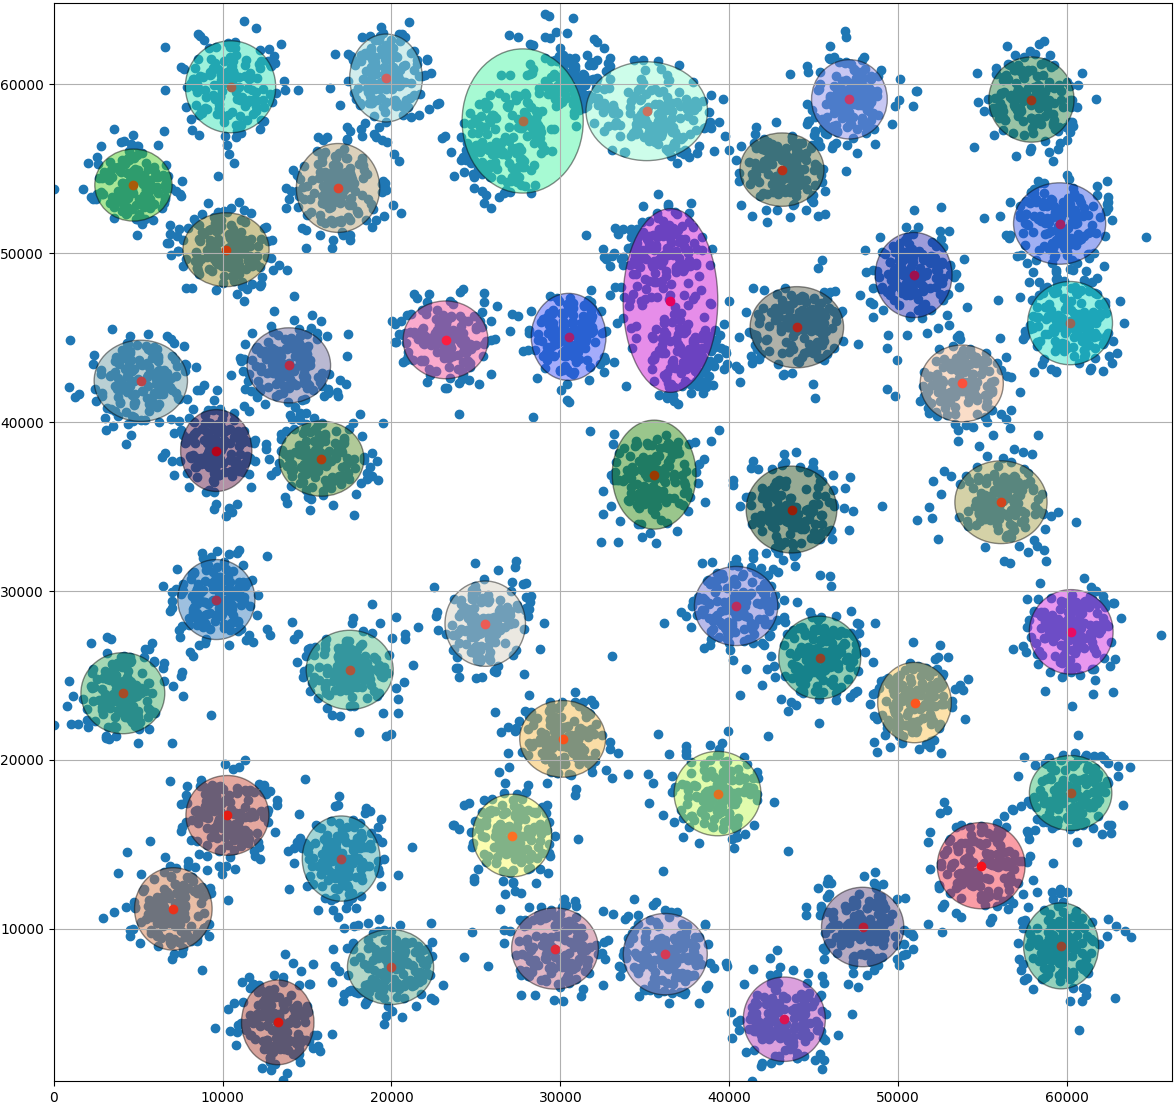
\includegraphics[width=0.5\textwidth]{a3_density_3.png}}
  \caption{The final outcome from a dataset with many small and dense regions.}
  \label{dataset1}
\end{figure}

\begin{figure}[t]
  \center{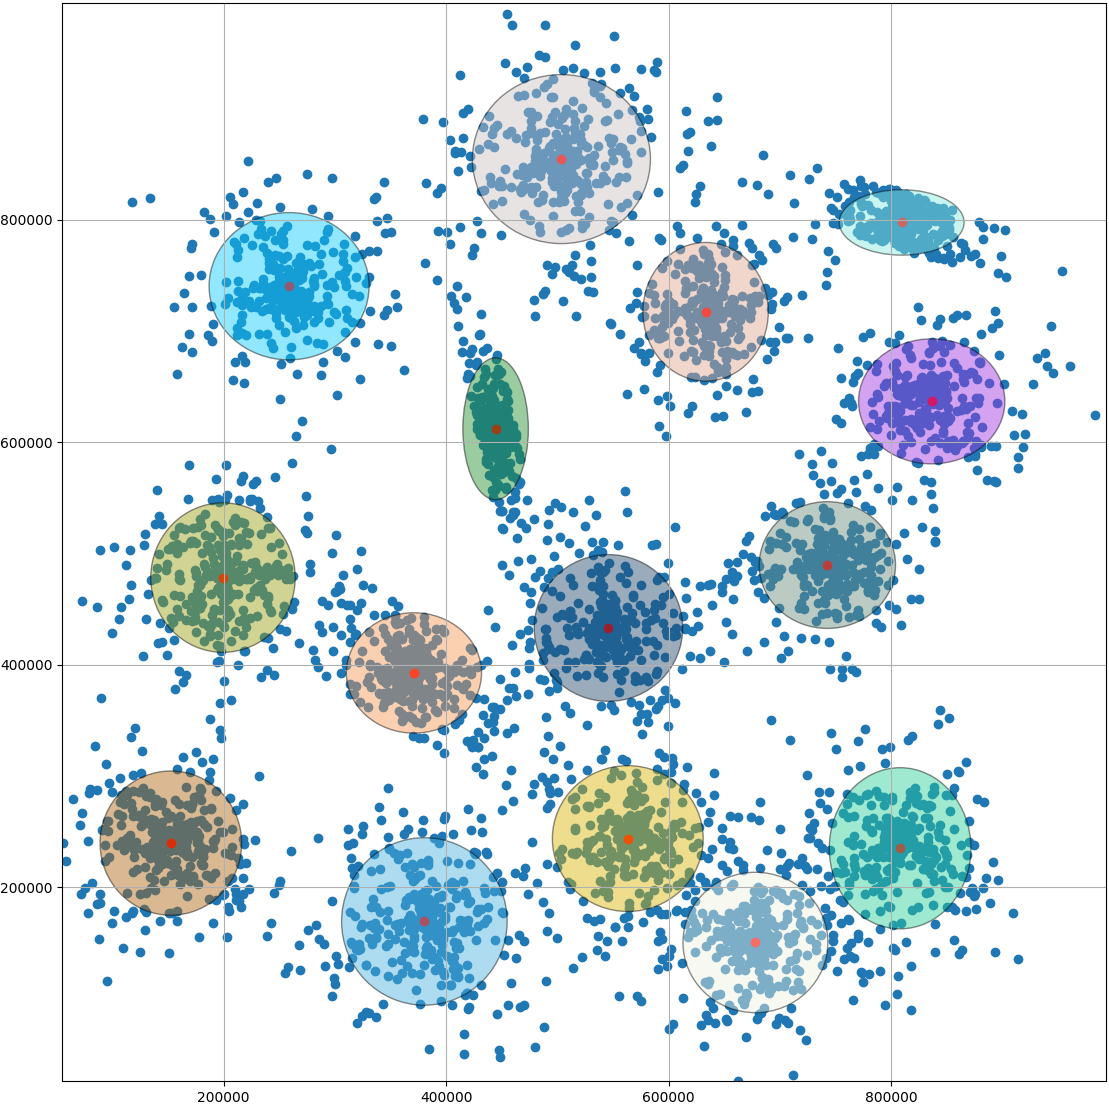
\includegraphics[width=0.5\textwidth]{s2_density_3.png}}
  \caption{The final outcome from a dataset with many small and quite sparse points.}
  \label{dataset2}
\end{figure}

\begin{figure}[t]
  \center{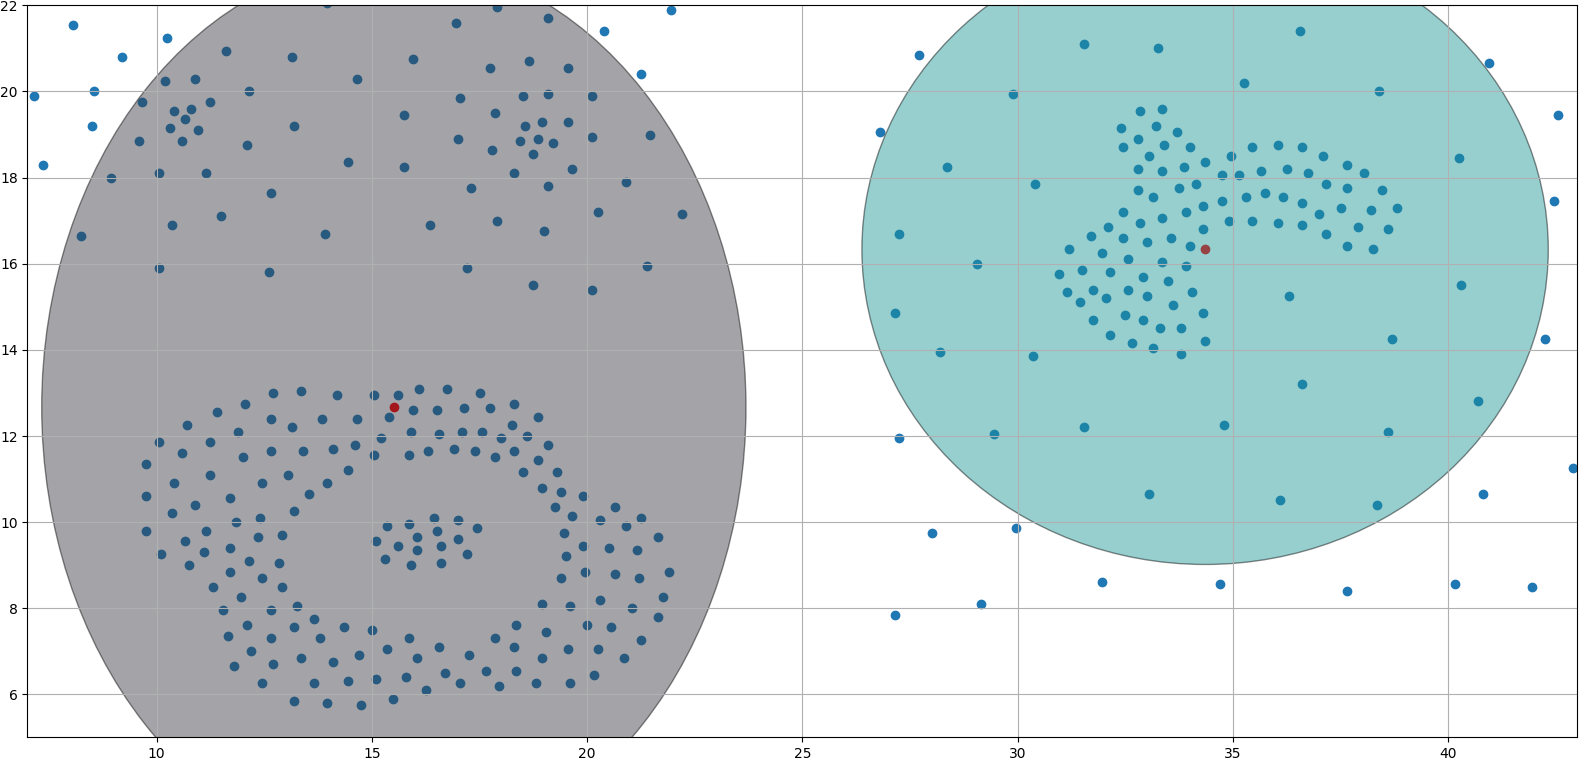
\includegraphics[width=0.5\textwidth]{Compound_density_1.png}}
  \caption{The final outcome from a very difficult dataset for a "k-means"-like algorithm.}
  \label{dataset3}
\end{figure}

As it is possible to see from Figure~\ref{dataset1} and \ref{dataset2}, this approach
succeeds in finding the right number of clusters and in positioning the centroids even
though the dataset cannot be considered an "easy" one. 
Furthermore, Figure~\ref{dataset3} highlights how a dataset that visually can be 
divided into few different shapes does not fit the capabilities of a partitioning
algorithm like the k-means to find the clusters. This is due to the underlying distribution
creating the points in the dataset that are far from being a smooth bell-curved shape.
This particular example is clearly crafted to hinder the clustering algorithm being tested.

However, the results displayed in this section clearly state that the approach developed
in this work provides good and promising results.
